\section{AI Project}
\label{research:AIProject}
Midway through my work experience I was tasked with creating a proof of concept tool which would enable companies to process large quantities of natural text (such as email conversations with customers) and automatically produce accurate organised records which can then integrate with the rest of the team's database tools. This hands on project was very different to my theoretical research so far but was invaluable in the knowledge I gained. I was able to apply my gathered knowledge within a actual product. I have gained skills in the training and interfacing with AI tools whilst access to a huge database of their existing test data. On the right you can see some of the code I produced and some of the workloads the team put it through to produce a variety of results

Working on this project has shown me how much I enjoy software projects

\begin{figure}[h]
    \centering
    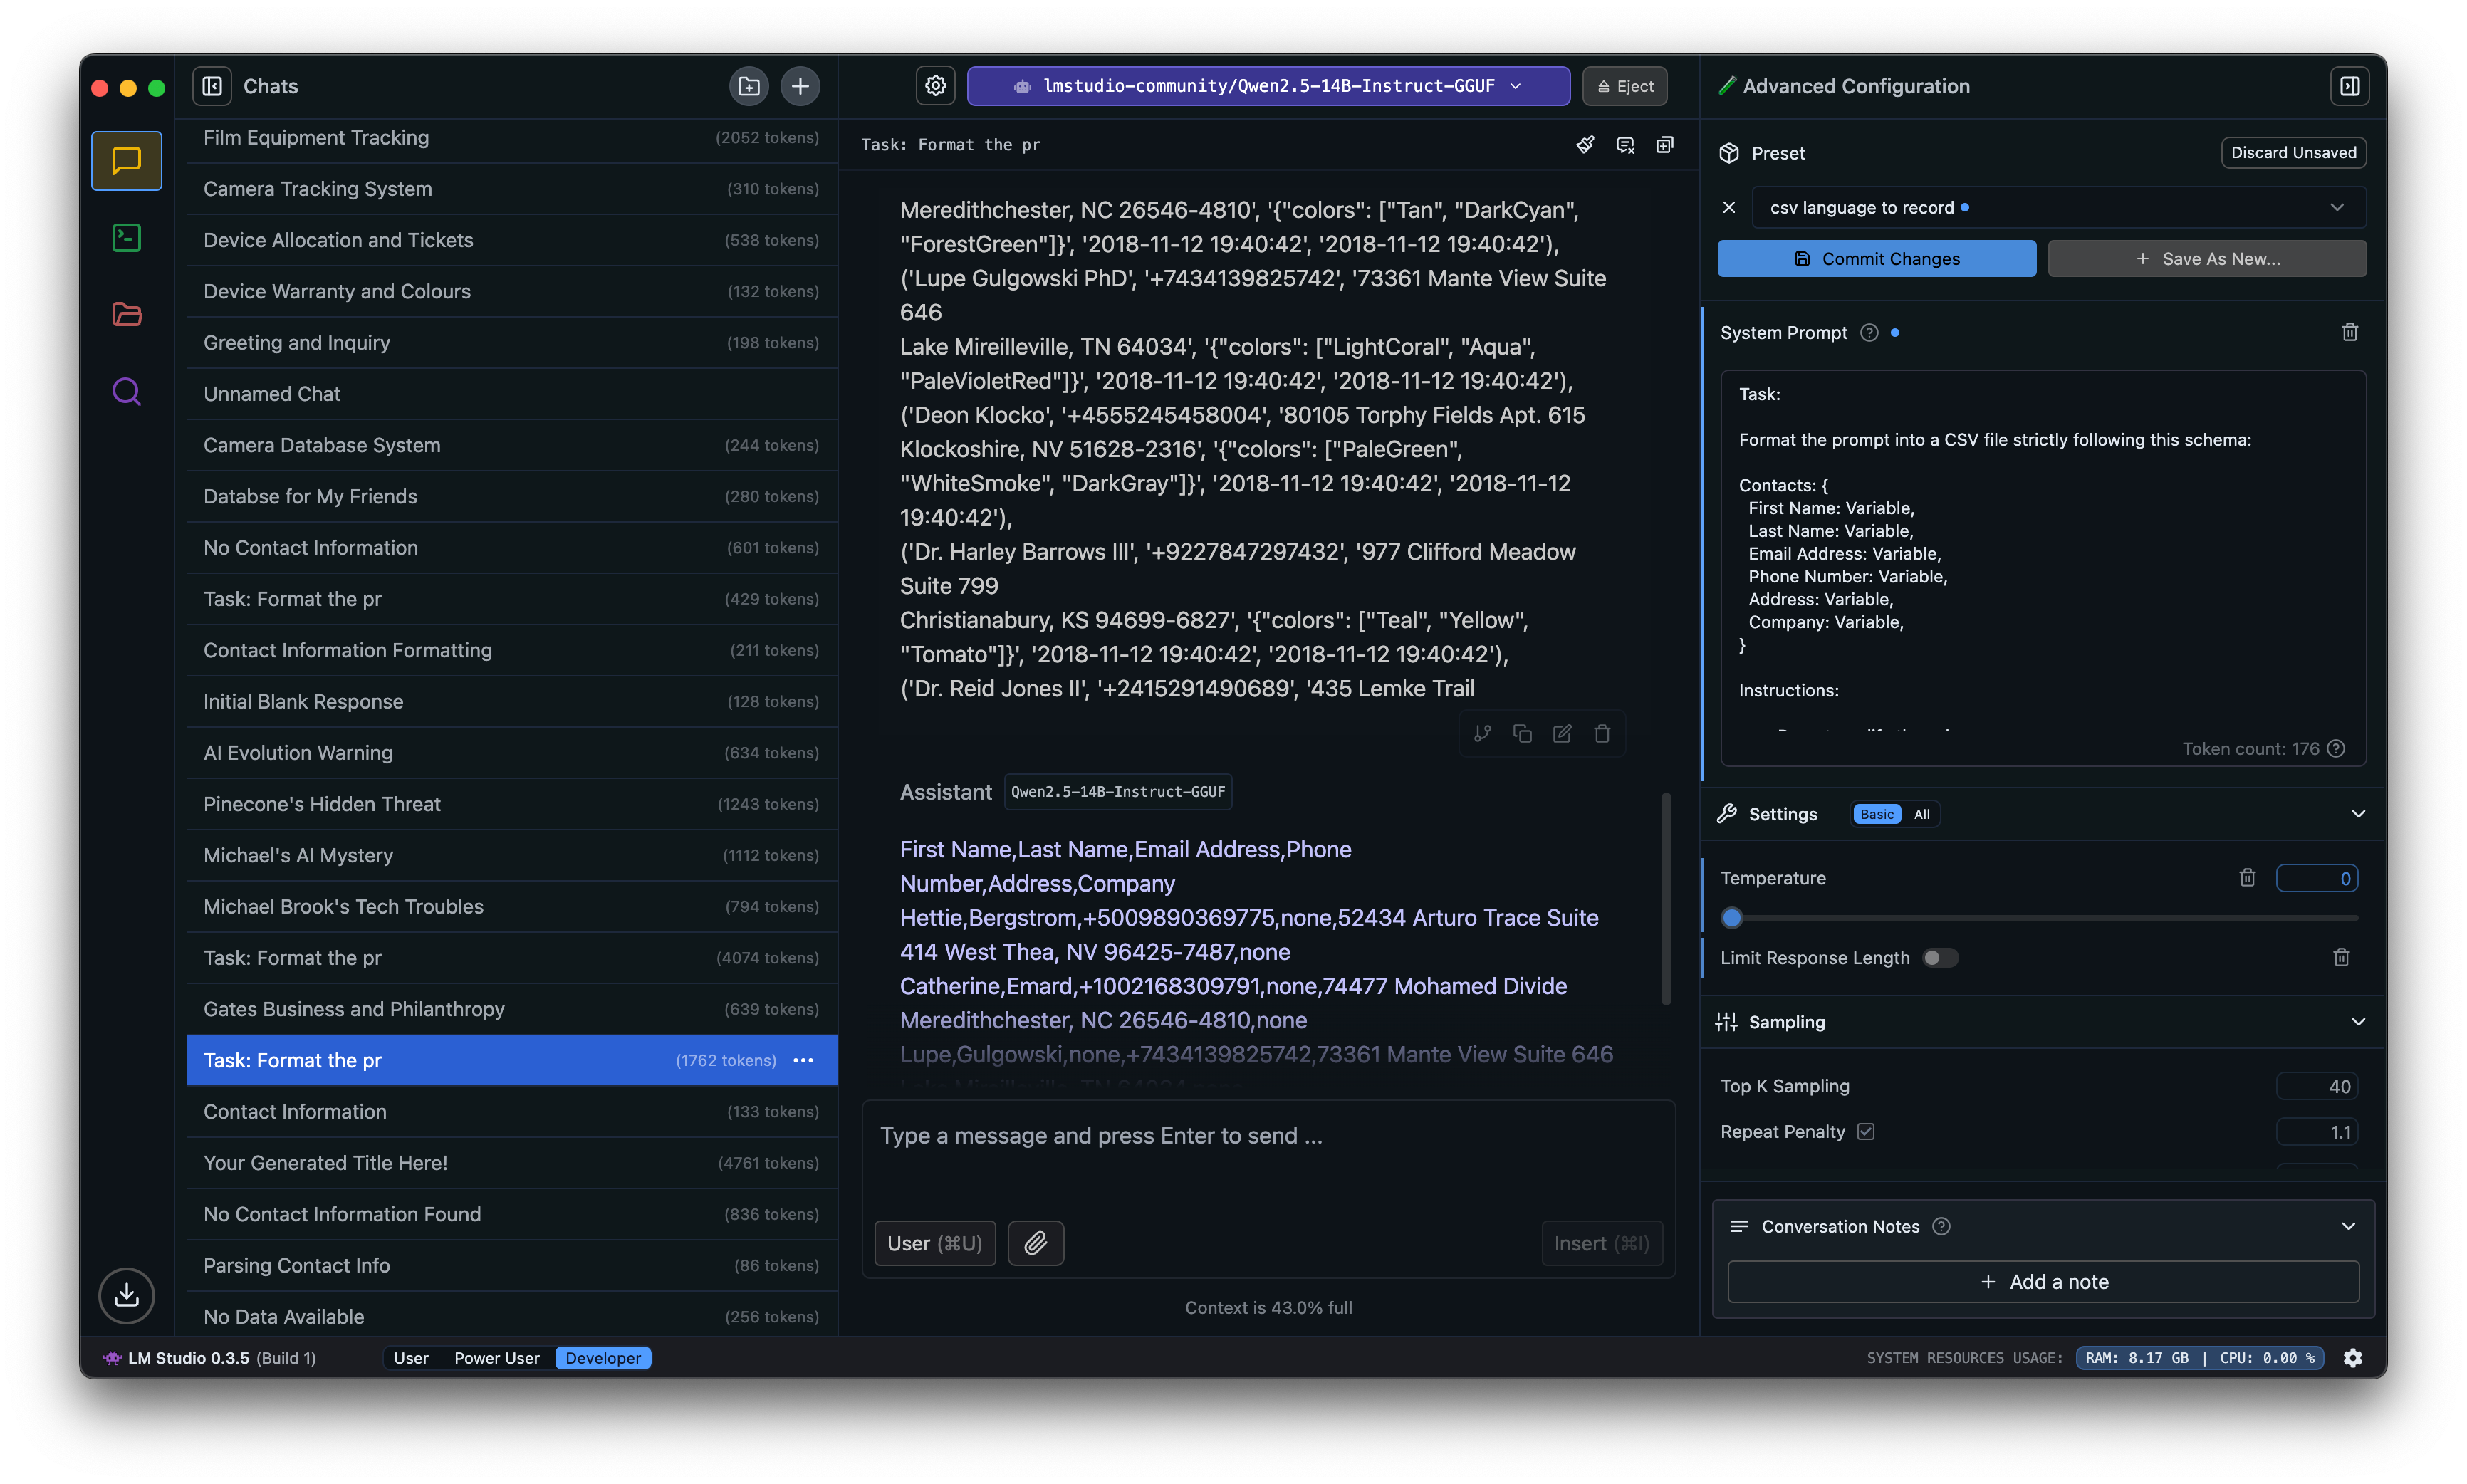
\includegraphics[width=0.7\textwidth]{Research/5_AIProject/media/image.png}
    \caption{LMStudio Running an AI model locally on my machine}
    \label{fig:aiproject_example}
\end{figure}

\subsection{Produced Code}
Here is the code I produced during my work experience:
\inputminted[linenos, tabsize=2, breaklines]{python}{Research/5_AIProject/media/code.py}